<<<<<<< HEAD
\section{Project Milestones}
In this project, we are aiming at implementing an automatic Ci generator with recurrent neural networks(RNN) that is able to learn the rules automatically and generate poems that are correct on grammar and meaningful. In addition, we would like to compare the performance of this generator with other algorithm, such as genetic algorithm\\

We plan to complete our project in the following four steps. Detailed project time line is showed in Figure \ref{fig:projecttimeline}:
=======
% !TEX root = /Users/zhuzhuangdi/Desktop/MSUCourses/MachineLearning847/17Project/17spr_wang_zhu_du/Proposal/main.tex
\section{Proposal Summary and Project Milestones}
In this project, we aim at implementing an automatic Song Ci generator to generate Song Ci poems that can satisfy grammar, rhythmic and poetic requirements.
%
We implement this generator using two approaches. First, we will implement it using recurrent neural networks.
%
Next, we would like to implement it with using genetic algorithms.
%
We will compare the performance of different generating algorithms.
%
We plan to complete our project in the following four steps:
and detailed project timeline is showed in Figure \ref{fig:projecttimeline}:
\begin{figure}[htbp]
	\centering
	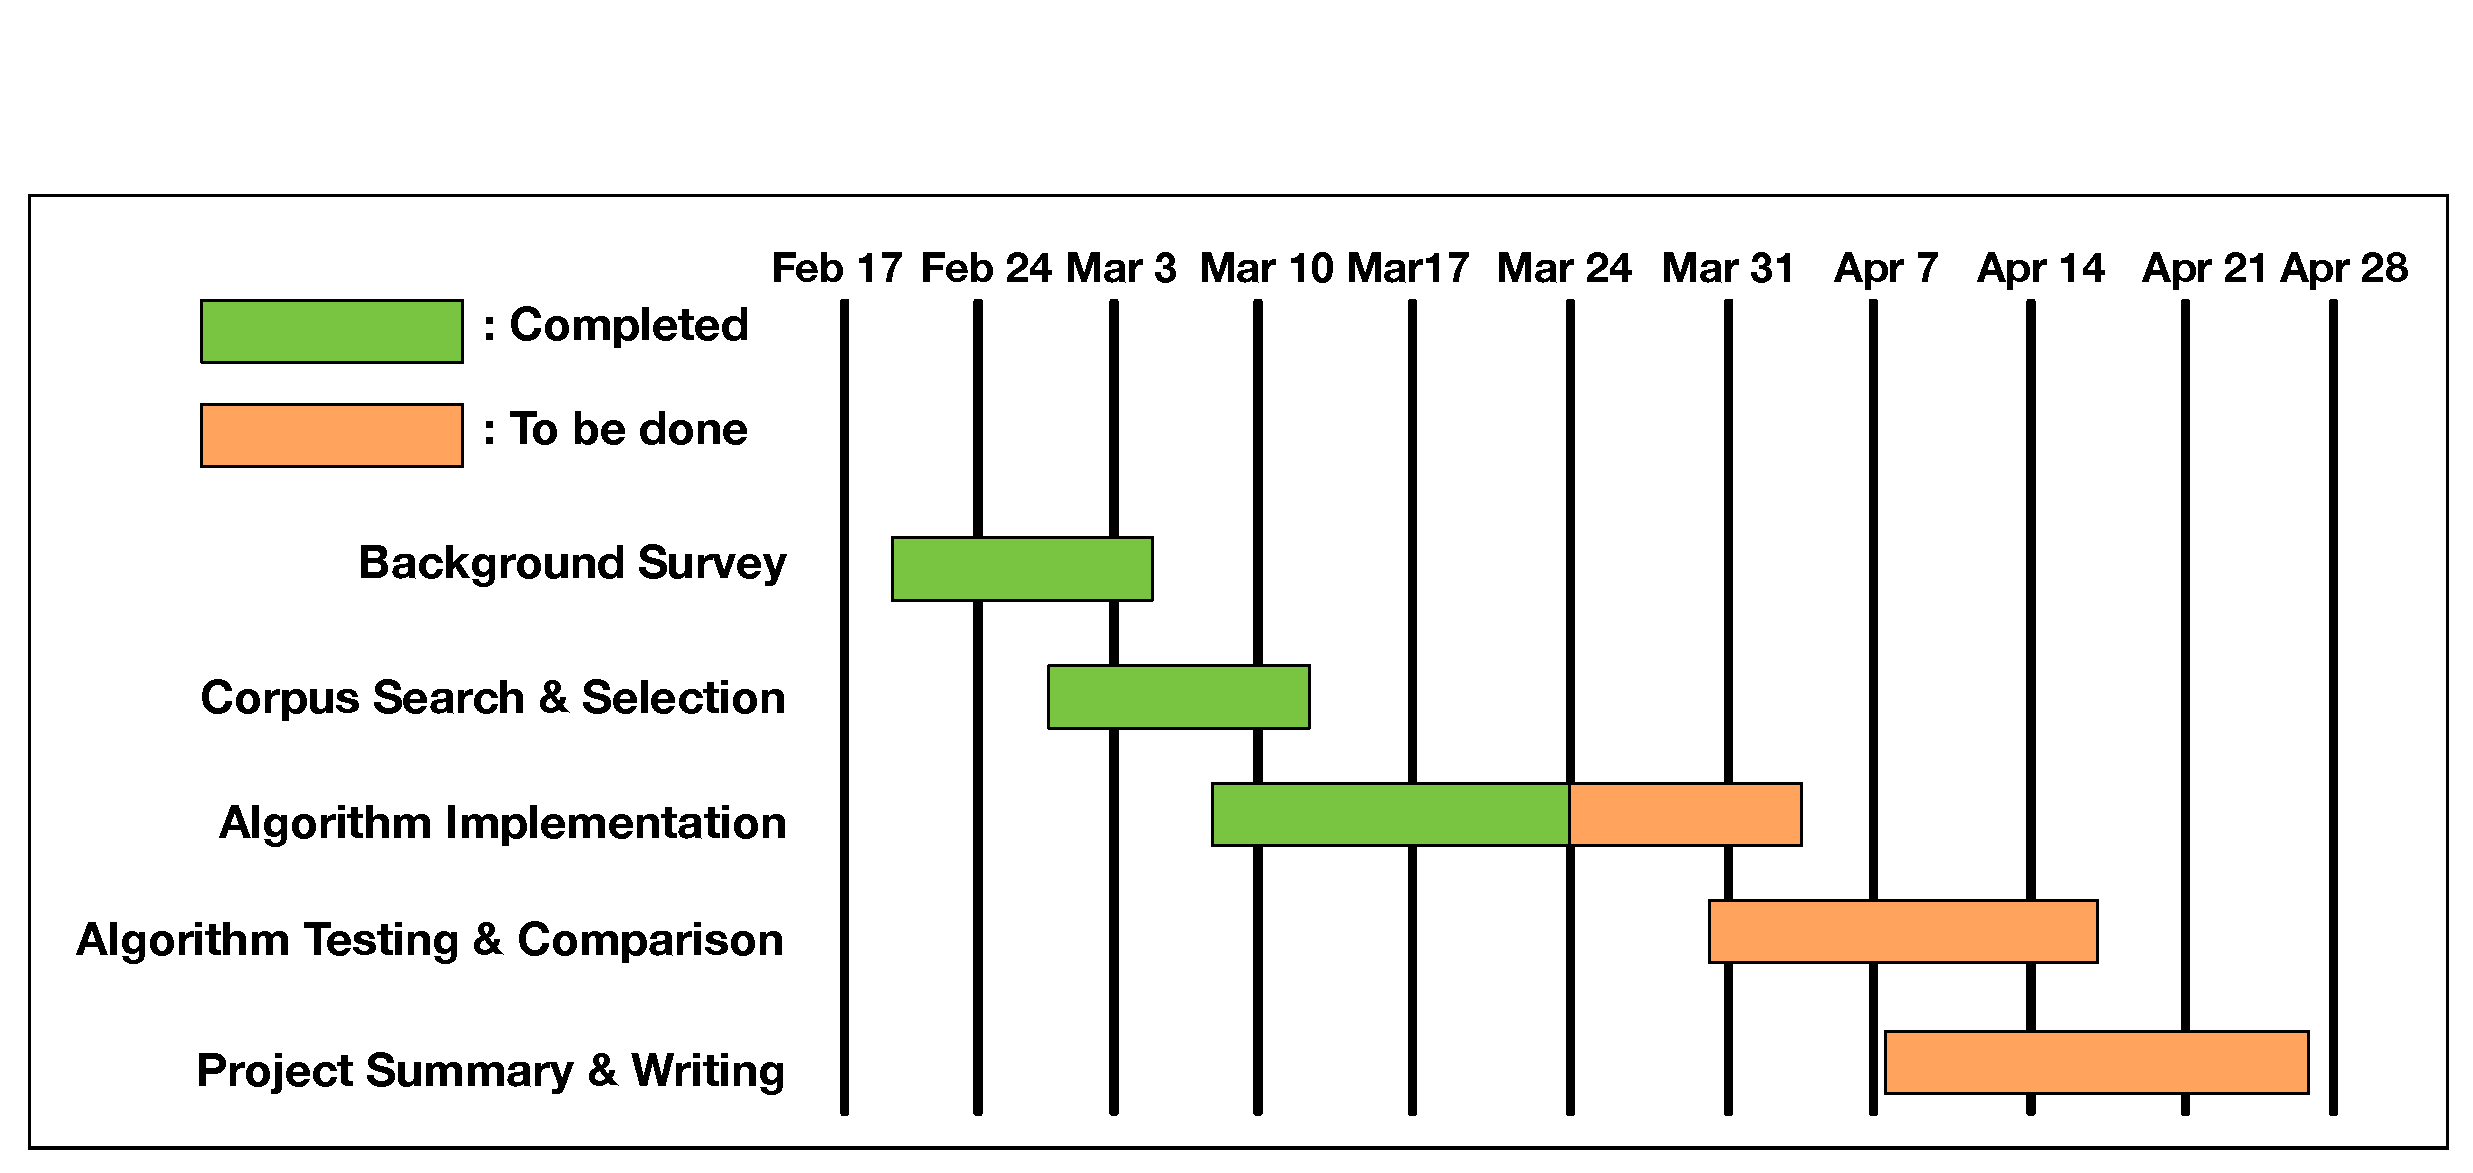
\includegraphics[width=0.9\linewidth]{mileStone}
	\caption{Project Timeline}
	\label{fig:projecttimeline}	
\end{figure}
>>>>>>> origin/master
\begin{itemize}
\item Background Survey
\item Corpus Search and Selection
\item Algorithm Implementation
\item Algorithm Testing and Comparison
\item Project Summary and Writing
\end{itemize}

For this initial step, we plan to search for related works to computational literary creation to gain the basic knowledge of Song Ci.
%
We are interested in the following questions: what is the criterion of a good Song Ci? How to evaluate the correctness, fluency and style of poems generated?
%
Better understanding of related work and Song Ci composition rules will provide us with great help for the following work, especially algorithm testing and comparison. 
%
Second, we will search and select a proper Song poem corpus for our project. The ideal corpus should be comprehensive on poem styles, and are precisely analyzed for content. 
%
Third, implementation poem generator based on both algorithm of RNN and genetic algorithm would be the most important work in our project. So we will assign more time on this step. 
%
Firth, test cases will be generated with both poem generator under the same keywords and topics. Poems will be test on aspects of grammar, semantic correctness, style and content. Both computational evaluation and human evaluation are expected to be used in last part of our project.


<<<<<<< HEAD
For the initial step, we plan to search for some related works on computational literary creation and gain insight into the basic knowledge of composition and appreciation of Ci Better understanding of related work and Ci composition rules will provide us great help for the following work, especially algorithm testing and comparison. Then, we will search and select a proper Ci corpus for our project. The ideal corpus should be comprehensive on Ci styles, and are precisely analyzed for content. Implementation poem generator based on both algorithm of RNN and traditional algorithm would be the most important work in our project. So we allocate more time on this step. Then test cases will be generated with both Ci generator under the same keywords and topics. Poems will be test on aspects of grammar, semantic correctness, style, content etc. Both computational evaluation and human evaluation are expected to be used in last part of our project.

=======
>>>>>>> origin/master
